\documentclass[a4paper]{article}
\usepackage{qtree}
\usepackage{forest}
\usepackage{multicol}
\setlength{\columnsep}{3cm}
\usepackage{parskip}
\usepackage{changepage}
\usepackage[T1]{fontenc}
\usepackage{amsmath}
\usepackage{listings}
\usepackage{amsthm}
\usepackage{amssymb}
\usepackage{float}
\usepackage[utf8]{inputenc}
\usepackage{graphicx}
\usepackage[italian]{babel}
\usepackage{thmtools}
\newtheorem*{theorem}{Teorema}
\newtheorem*{definition}{Definizione}
\newtheorem{example}{Example}
\newenvironment{dimostrazione}{\textit{Dimostrazione}:\begin{adjustwidth}{2cm}{}}{\end{adjustwidth}}

\begin{document}

\author{Lorenzo Dentis, lorenzo.dentis@edu.unito.it}
\title{Risposte AlgComp}
\maketitle

\section{Brute-force e certificazione}
\subsection{A.1}
Posto un array $V$ di $n$ elementi individuo due indici, $i$ e $j$.\\L'idea è di mantenere gli elementi $[0 ... j-1]$ fissi ed andare a generare tutte le permutazioni dei restanti elementi $[j ... n-1]$grazie all'indice $i$.

Ad ogni incremento dell'indice $i$ segue una sequenza di chiamate ricorsive che hanno lo scopo di effettuare uno swap fra l'elemto di indice $i$ e l'elemento di indice $j$ e poi incrementare $j$ scendendo nell'albero della ricorsione fino alla condizione $j=i$, quando $i$ viene di nuovo incrementato.Intuitivamente $j$ indica la profondità della ricorsione, $i$ indica l'ampiezza.
\begin{itemize}
	\item \textbf{Punto 1}:L'algoritmo è completo in quanto genera $n!$ permutazioni, ed è corretto in quanto sono tutte distinte.\\Le permutazioni generate sono esattamente $n!$ in quanto alla "radice" dell'albero avrò $n$ chiamate ricorsive (con $i = 0, i=1, ... i= n-2, i=n-1$ ).Invece al livello di profondità $j$ i primi $j$ elementi del vettore risulteranno fissi ed avrò solo $n-1-j$ chiamate ricorsive.\\Considerando che il valore di $j$ viene incrementato di una unità ad ogni "livello" di ricorsione fino all' $n-(n-1)$esimo livello ottengo questa semplice equazione: \begin{center}$calls = n * (n-1) * ...(j-1$volte$)... * 1$\end{center}Che non è altro che $n!$\\
		Le permutazioni sono tutte distinte perchè $i$ e $j$ non assumono mai due volte lo stesso valore, posto che ogni elemento del vettore sia distinto.Di conseguenza lo "swap" avverrà sempre tra due elementi differenti ad ogni chiamata ricorsiva, generando sottoalberi uno diverso dall'altro e di conseguenza sequenze differenti.
	\item \textbf{Punto 2}:Un algoritmo che generi \textit{tutti i sottoinsiemi di elementi} può essere realizzato organizzando lo spazio degli stati in sottoinsiemi.
		Al posto che intendere una permutazione come sequenza di elementi la si può vedere come una serie di \textit{scelte}, ovvero booleani.Essenzialmente si va a generare un vettore $B$ di booleani i cui elementi indicano se il corrispondente elemento di $V$ va considerato o meno.\\
		Se $B[i] == True$ allora $V[i]$ fa parte del sottoinsieme che si sta generando.\\
		In tal modo otteniamo il \textbf{PowerSet} di $V$, che è completo (cioè le permutazioni sono $2^n$) in quanto ogni cella del vettore $B$ può avere solamente valore binario e le celle sono $n$.
		E' invece corretto, di nuovo posto che gli elementi siano distinti, in quanto non vi è alcuno \textit{"swap"} e nessuna sequenza è ripetuta più volte. Ogni sequenza di \textit{True/False} varia dalla precedente di una scelta, garantendo sequenze distinte.
\end{itemize}
\begin{figure*}[!ht]
\centering
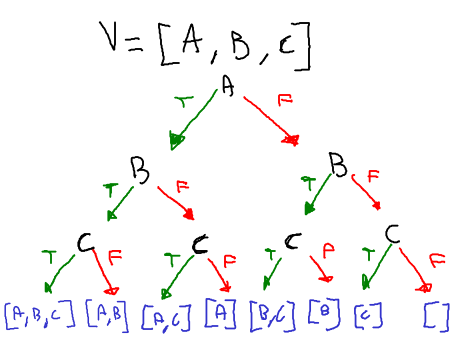
\includegraphics[scale = 0.5]{./img/A1_2.png}
\caption{PowerSet di [a,b,c]} \label{FIG:PowerSet}
\end{figure*}
\subsection{A.2}
Definizione formale di una permutazione (definizione ricorsiva):
\begin{figure*}[!ht]
\centering
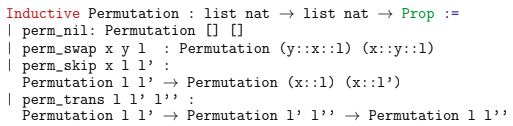
\includegraphics[width=0.7\textwidth]{./img/permutazione_ricorsiva.png}
\caption{Definizione ricorsiva di una permutazione} \label{FIG:recursive_permutation1}
\end{figure*}
\begin{itemize}
	\item perm\_nil: [ ] è permutazione di [ ] (lista vuota è permutazione di se stessa)
	\item perm\_swap: $\forall x,y \in Elements$ e $\forall l \in Lists$ $[y::x::l]$ e $[x::y::l]$ sono una permutazione dell'altra
	\item perm\_skip: dato $x \in Elements$, se $l \in Lists$ è permutazione di $l' \in Lists$ $\Rightarrow [x::l]$ è permutazione di $[x::l']$
	\item perm\_trans: date $l, l', l'' \in Lists$ se $l$ permutazione di $l'$ e $l'$ permutazione di $l'' \Rightarrow l$ è permutazione di $l''$ 
\end{itemize}
\begin{theorem}[Riflessività] $\forall l \in Lists$ Permutation $l$ $l$\end{theorem}
\textit{Dimostrazione}:
\begin{adjustwidth}{2cm}{}
	\textit{caso base}: $l$ = [ ], vale per definizione grazie a perm\_nil\\
	\textit{caso induttivo}: $l = [h::t]$ con $h \in Lists$ e $t \in ELements$.\\
	Grazie all'ipotesi induttiva si può affermare \textit{Permutation} $t$ $t$ e quindi per perm\_skip \textit{Permutation} $[h::t]$ $[h::t]$. Dato che $l = [h::t]$ abbiamo che \textit{Permutation} $l$ $l$.
\end{adjustwidth}
\begin{theorem}[Simmetria] $\forall l,l' \in Lists$, Permutation $l$ $l'$ $\Rightarrow $ Permutation $l$ $l'$\end{theorem}
\begin{dimostrazione}
	DA FAR
\end{dimostrazione}
\subsection{A.3}
Dimostrare che è algoritmo che genera permutazioni di una lista di elementi è completo significa dimostrare che genera $n!$ permutazioni, con $n$ pari al numero di elementi. Formalmente:
\begin{theorem}[Completezza] $\forall l \in Lists$, $len($\textit{permutation} $l) = len(l)!$\end{theorem}
\begin{dimostrazione}
	\textit{caso base}: $l$ = [ ]\\
	In questo caso $len(l)! = 0! = 1$.\\
	Allo stesso modo $len(permutation)$ [ ] $= len($[ [ ] ]$) = 1$.\\
	Quindi $len($\textit{permutation} $l) = len(l)!$
	
	\textit{Caso induttivo}: $l = h::t$, quindi l'enunciato da dimostrare è $len($\textit{permutation} $[h::t]) = len([h::t])!$\\
	$len(h::t) = 1 + len(t)$\\
	Quindi $len(distribute$ $a$ $[h::t]) = 2 + len(t)$ che per il Lemma distribute\_lenght diventa $len((a::t)::distribute$ $a$ $t) = 2 + len(t)$
	INSERIRE FOTO LEMMA DISTRIBUTE
\end{dimostrazione}
\subsection{A.4}
\begin{itemize}
	\item \textbf{Permutazioni}:Si può individuare una \emph{risposta} al problema \textbf{Valutazione} generando l'albero di tutte le possibili permutazioni:
		\begin{center}	\Tree [  [ [ .1 [  [ .2 [.3 4 ] [.4 3 ] ] [ .3 [.2 4 ] [ .4 2 ] ] [ .4 [ .2 3 ] [ .3 2 ] ] ] ] [ .2 [ [ .1 [ .3 4 ] [ .4 3 ] ] [ .3 [ .1 4 ] [ .4 1 ] ] [ .4 [ .1 3 ] [ .3 1 ] ] ] ] [ .3 [ [ .1 [ .2 4 ] [ .4 2 ] ] [ .2 [ .1 4 ] [ .4 1 ] ] [ .4 [ .1 2 ] [ .2 1 ] ] ] ] [ .4 [ [ .1 [ .3 2 ] [ .2 3 ] ] [ .3 [ .1 2 ] [ .2 1 ] ] [ .2 [ .1 3 ] [ .3 1 ] ] ] ] ] ]
		\end{center}
		In questo albero un ramo individua una permutazione dell'insieme di partenza, di conseguenza basta percorrerlo calcolando di volta in volta il voto massimo finchè questi non supera il valore fissato (in questa istanza 9).Si ottiene quindi una soluzione, data dalla sequenza di "voti" ottenuta partendo dalla radice e percorrendo il ramo corrispondente fino al padre del nodo che causa il superamento del voto massimo.
		Eseguendo questa operazione su tutti i rami dell'albero si ottengono tutte le \emph{soluzioni}, scegliendo le soluzioni con votazione migliore si ottengono una o più \emph{risposte}.
	\item \textbf{Sottoinsiemi}:Si può individuare una \emph{risposta} al problema \textbf{Valutazione} generando l'albero di tutte le possibili scelte:
		\begin{center}
			\begin{forest}
				for tree={ l sep=20pt, s sep=20pt}
			[1 [2, edge label = {node[midway,left,green] {T}} [3, edge label = {node[midway,left,green] {T}}[4, edge label = {node[midway,left,green] {T}}] [4, edge label = {node[midway,right,red] {F}}]] [3, edge label = {node[midway,right,red] {F}}[4, edge label = {node[midway,left,green] {T}}] [4, edge label = {node[midway,right,red] {F}}]]][2, edge label = {node[midway,right,red] {F}} [3, edge label = {node[midway,left,green] {T}}[4, edge label = {node[midway,left,green] {T}}] [4, edge label = {node[midway,right,red] {F}}]] [3, edge label = {node[midway,right,red] {F}}[4, edge label = {node[midway,left,green] {T}}] [4, edge label = {node[midway,right,red] {F}}]]]] 			\end{forest}
		\end{center}
		A seconda che si scelga un ramo o l'altro la domanda sarà inclusa nella possibile \emph{soluzione} quindi percorrendo un ramo fino alla foglia si giunge sempre ad una sequenza di voti.
		Non tutti i sottoinsiemi così generati sono però \emph{soluzioni}, in quanto alcuni superano il vincolo del voto massimo ammesso (in questo caso 9); considerando solo le \emph{soluzioni} e scegliendo quelle aventi la migliore votazioni si ottengono una o più \emph{risposte}
\end{itemize}
\section{Backtrack}
\section{Branch\&Bound}
\subsection{C.7}
Guarda la scacchiera come una matrice di 1 e 0
\end{document}
